
%(BEGIN_QUESTION)
% Copyright 2007, Tony R. Kuphaldt, released under the Creative Commons Attribution License (v 1.0)
% This means you may do almost anything with this work of mine, so long as you give me proper credit

The following storage vessel holds acetone, a liquid with a density of 49.4 lb/ft$^{3}$.  A pressure transmitter located 4 feet below the vessel bottom infers acetone level by hydrostatic pressure (head).  Determine the calibration range of this pressure transmitter in order to properly translate the range of vessel level (0 to 14 feet) into an output signal of 4 to 20 mA.  Please express the transmitter's calibration range in units of kPa.

$$\includegraphics[width=15.5cm]{i02962x01.eps}$$

Then, determine the following (assuming the transmitter has been properly calibrated for the application):

\begin{itemize}
\item{} Transmitter output signal (mA) at 5.2 feet of level
\item{} Acetone level at 12.7 mA signal output
\end{itemize}

\underbar{file i02962}
%(END_QUESTION)





%(BEGIN_ANSWER)

Lower range-values (LRV): 9.461 kPa input = 4 mA output

\vskip 10pt

Upper range-values (URV): 42.57 kPa input = 20 mA output

\vskip 10pt

\begin{itemize}
\item{} Transmitter output signal (mA) at 5.2 feet of level = 9.943 mA
\item{} Acetone level at 12.7 mA signal output = 7.613 feet
\end{itemize}

%(END_ANSWER)





%(BEGIN_NOTES)


%INDEX% Measurement, level: hydrostatic pressure

%(END_NOTES)


